% ============================================================
%  Figure 13 — Normalised condition number vs window length
%  Log y-axis
% ============================================================
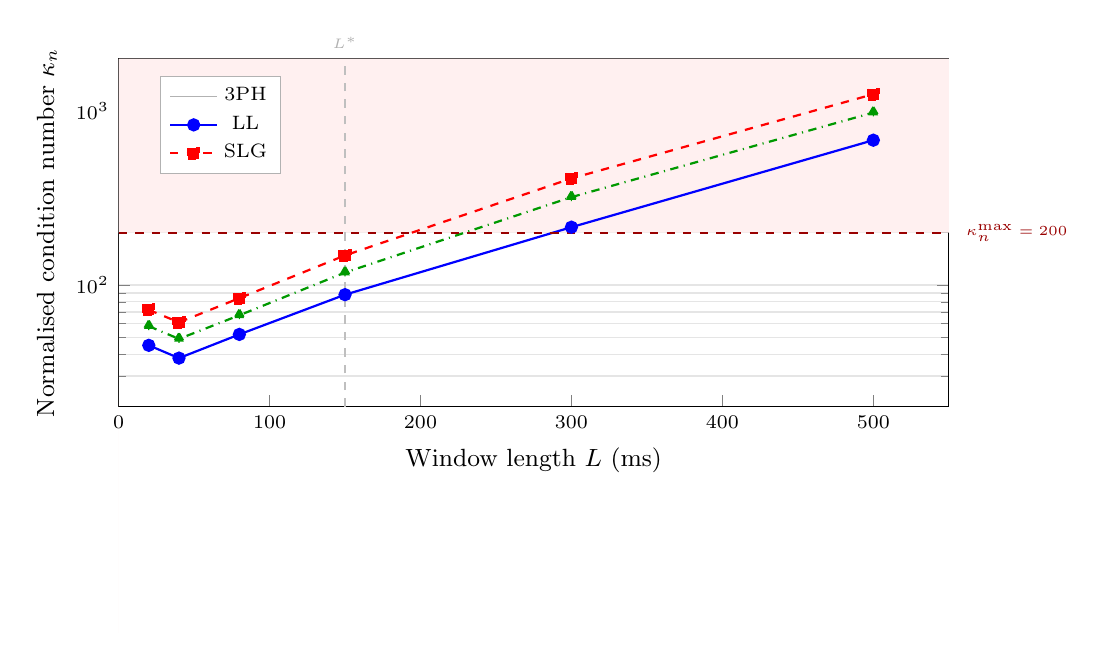
\begin{tikzpicture}
\begin{axis}[
  width=\columnwidth, height=6.0cm,
  xlabel={Window length $L$ (ms)},
  ylabel={Normalised condition number $\kappa_n$},
  xmin=0, xmax=550, ymin=20, ymax=2000,
  xtick={0,100,200,300,400,500},
  ymode=log,
  ymajorgrids=true, yminorgrids=true,
  grid style={gray!20},
  label style={font=\small},
  tick label style={font=\scriptsize},
  legend style={at={(0.05,0.95)}, anchor=north west,
                font=\scriptsize, fill=white, draw=black!30},
  clip=false
]

% Shaded ill-conditioning region κ_n > 200
\addplot[fill=red!6, draw=none]
  coordinates {(0,200)(550,200)(550,2000)(0,2000)} \closedcycle;

% 3PH
\addplot[blue, solid, thick, mark=*, mark size=2pt] coordinates {
  (20,45)(40,38)(80,52)(150,88)(300,215)(500,680)
};
% LL
\addplot[red, dashed, thick, mark=square*, mark size=2pt] coordinates {
  (20,72)(40,61)(80,84)(150,148)(300,410)(500,1250)
};
% SLG
\addplot[green!60!black, dashdotted, thick, mark=triangle*, mark size=2pt] coordinates {
  (20,58)(40,49)(80,67)(150,118)(300,320)(500,980)
};

% Ill-conditioning threshold κ_n = 200
\draw[thick, red!60!black, dashed]
     (axis cs:0, 200) -- (axis cs:550, 200);
\node[right, font=\tiny, red!60!black]
     at (axis cs:555, 200) {$\kappa_n^{\max}=200$};

% Validity boundary
\draw[thick, gray!50, dashed]
     (axis cs:150, 20) -- (axis cs:150, 2000);
\node[above, font=\tiny, gray!60] at (axis cs:150, 2000) {$L^*$};

\legend{3PH, LL, SLG};

\end{axis}
\end{tikzpicture}
